\chapter{Dataset Construction}
\label{cha:dataset}

The benchmark of this thesis rests on a dataset that did not previously exist in the form
required: a single table pairing measured photovoltaic power, weather and solar-geometry
covariates, and co-registered satellite imagery, across two regions, at native cadence,
with plant identity as the split key. This chapter states the requirements that shaped it,
the sources fused, the harmonisation performed, the resulting schema, the quality flags,
and the plant-disjoint partition used everywhere in Chapters~\ref{cha:baselines}
and~\ref{cha:expdesign}.

\section{Design requirements}
\label{sec:data-requirements}

Five requirements were fixed before construction, each of which excludes a common shortcut.

\begin{enumerate}
  \item \textbf{One row per (plant, timestamp).} Power, covariates and a frame pointer live
    on the same row. This makes windowing a slicing operation and removes any possibility
    of misalignment between modalities.
  \item \textbf{Native cadence, no resampling.} The two source datasets sample at 30 and 15
    minutes. Resampling to a common grid would either discard information or fabricate it;
    instead, windows are defined in \emph{physical time} and resolved to a different number
    of steps per dataset (Section~\ref{sec:windows}).
  \item \textbf{No gap interpolation beyond a strict threshold.} Long gaps are dropped
    rather than filled, so that a model is never scored against invented targets.
  \item \textbf{Plant identity as the split key.} Every row carries \texttt{site\_id}, and
    splits partition plants, never timestamps.
  \item \textbf{Frames addressable in constant time.} Millions of individual image files
    are impractical on a shared cluster filesystem; frames are packed into one HDF5 archive
    with a direct integer pointer from each table row.
\end{enumerate}

\section{Sources}
\label{sec:sources}

Four public sources are fused. Table~\ref{tab:sources} summarises what each contributes.

\begin{table}[h!]
\centering
\small
\begin{tabular}{p{2.6cm} p{4.4cm} p{6.2cm}}
\hline
\textbf{Track} & \textbf{Source} & \textbf{Contribution} \\
\hline
PV power, UK & \texttt{openclimatefix/uk\_pv}~\cite{ukpv} & 30-minutely domestic
generation, 2019--2020, with per-site metadata: rounded latitude/longitude and nameplate
capacity in kWp. \\
Imagery, UK & EUMETSAT SEVIRI RSS, high-resolution visible channel~\cite{eumetsat} &
Approximately 1\,km per pixel, reprojected to each site and cropped to
$128\times128$ pixels ($\approx$128\,km), sized for cloud-advection context. \\
PV power and imagery, US & NREL PVDAQ via the OEDI data lake~\cite{pvdaq}, paired with
GOES-16 crops & 10 sites with site metadata (coordinates, nameplate power) and
$256\times256$ RGB satellite crops. \\
Weather & Open-Meteo Archive API~\cite{openmeteo} & Eight hourly variables per site:
2\,m temperature, shortwave / direct / diffuse radiation, direct normal irradiance, cloud
cover, 10\,m wind speed, precipitation. \\
\hline
\end{tabular}
\caption{The four public sources fused into the dataset of record.}
\label{tab:sources}
\end{table}

\section{Harmonisation}
\label{sec:harmonisation}

\paragraph{Power.} UK generation is published as energy over a 30-minute interval
(\texttt{generation\_Wh}) and is converted to instantaneous power in watts by a factor of
two. Gaps of at most three steps are linearly interpolated; longer gaps are dropped rather
than filled. Nameplate capacity is audited per site and stored as
\texttt{installed\_power\_w}; the modelling target is
\[
  \texttt{norm\_power} = \frac{\texttt{power\_w}}{\texttt{installed\_power\_w}} \in [0,1],
\]
set to \texttt{NaN} on rows flagged as outage or stuck. Capacity normalisation is what makes
a 1.5\,kW rooftop and a 408\,kW utility array commensurable, and --- critically for the
cross-plant protocol --- it uses a quantity known at installation rather than a statistic
estimated from the measured signal.

\paragraph{Weather.} The eight Open-Meteo variables are hourly, while the power tracks are
sub-hourly; they are joined to each row by nearest timestamp using an as-of merge, so a
30-minute row inherits the enclosing hour's reanalysis values.

\paragraph{Solar geometry and clear-sky quantities.} Deterministic quantities are derived
per row from coordinates and timestamp: solar zenith and azimuth, a Haurwitz clear-sky
global horizontal irradiance model~\cite{haurwitz}, the clearness index $k_t$, the clear-sky
index (undefined and left as \texttt{NaN} below 50\,W/m$^2$ of clear-sky irradiance),
sine and cosine day-of-year encodings, and local apparent solar time. These are the only
covariates that are legitimately \emph{known in advance} over the forecast horizon; the
distinction is what separates the honest and oracle variants of the foundation-model
baselines in Section~\ref{sec:parity}.

\paragraph{Frames.} Per frame, missing values are set to zero, values are clipped to
$[0,1]$, and empty crops are discarded. Frames are written as a single \texttt{uint8} HDF5
archive rather than as individual files.

\section{Storage layout and the frame pointer}
\label{sec:layout}

The result is two artefacts:

\begin{itemize}
  \item \texttt{dataset\_all.parquet} --- $1{,}337{,}654$ rows $\times$ 35 columns, covering
    both datasets;
  \item \texttt{images\_all.h5} --- 27\,GB, 110 per-site HDF5 groups named
    \texttt{<dataset>\_<site>}, each holding an \texttt{images} array and a
    \texttt{timestamps} array of ISO-8601 byte strings.
\end{itemize}

Alignment between the two is carried by a single canonical column,
\texttt{image\_h5\_index}. It is a \emph{group-local} index into
\texttt{images\_all.h5[<dataset>\_<site>]["images"]} --- not a global row number --- and it
is timestamp-exact, verified row by row for both datasets. This deserves emphasis because
the table retains two legacy pointer columns: \texttt{image\_index}, which approximates the
canonical pointer, and \texttt{image\_uk128\_index}, which is dead and points into a file
that no longer exists. Any re-use of this dataset should read frames exclusively through
\texttt{image\_h5\_index}.

A visual step is considered valid --- the mask $\texttt{mask\_visual}=1$ --- if and only if
the row has a matching pointer and timestamp. Night and outage steps have no frame, which
means the visual mask is structurally correlated with the diurnal cycle; models must handle
this rather than assume a dense visual stream.

\section{Schema}
\label{sec:schema}

Table~\ref{tab:schema} groups the 35 columns by role.

\begin{table}[h!]
\centering
\small
\begin{tabular}{p{3.0cm} p{10.5cm}}
\hline
\textbf{Group} & \textbf{Columns} \\
\hline
Identity & \texttt{dataset}, \texttt{site\_id}, \texttt{station\_id},
\texttt{camera\_id}, \texttt{timestamp\_utc}, \texttt{latitude}, \texttt{longitude} \\
Target & \texttt{power\_w}, \texttt{installed\_power\_w}, \texttt{norm\_power} \\
Weather covariates & \texttt{temperature\_2m}, \texttt{shortwave\_radiation},
\texttt{direct\_radiation}, \texttt{diffuse\_radiation},
\texttt{direct\_normal\_irradiance}, \texttt{cloudcover}, \texttt{windspeed\_10m},
\texttt{precipitation} \\
Solar geometry and clear-sky & \texttt{solar\_zenith}, \texttt{solar\_azimuth},
\texttt{clearsky\_ghi}, \texttt{kt}, \texttt{csi}, \texttt{doy\_sin}, \texttt{doy\_cos},
\texttt{solar\_time} \\
Quality flags & \texttt{capacity\_fixed}, \texttt{outage\_flag}, \texttt{stuck\_flag},
\texttt{night\_clamped}, \texttt{bad\_site\_flag} \\
Frame pointers & \texttt{image\_h5\_index} (canonical), \texttt{image\_index},
\texttt{image\_path} \\
\hline
\end{tabular}
\caption{Column groups of \texttt{dataset\_all.parquet}.}
\label{tab:schema}
\end{table}

\section{Quality flags and curation}
\label{sec:quality}

Curation is recorded as flags rather than applied destructively, so that any downstream
decision to include or exclude a row is visible and reversible.

\begin{itemize}
  \item \texttt{bad\_site\_flag} --- whole sites whose series is unusable: \texttt{uk\_pv}
    sites 7239 and 8587, \texttt{goes\_pvdaq} sites 1283 and 51.
  \item \texttt{outage\_flag} --- 15{,}486 rows with zero or anomalous output during
    daylight.
  \item \texttt{stuck\_flag} --- 1{,}318 rows where the sensor reports a constant value
    across a period during which it should have varied.
  \item \texttt{night\_clamped} --- 1{,}535 rows where night-time output was clamped to
    zero.
\end{itemize}

One inconsistency is recorded here rather than concealed: the committed
\texttt{goes\_pvdaq} split predates the introduction of \texttt{bad\_site\_flag} and still
assigns sites 1283 and 51 to train and validation respectively. That split must be
regenerated, excluding the two flagged sites and leaving eight usable plants, before the
\texttt{goes\_pvdaq} track is run. No result reported in this thesis is affected, because
every reported run is restricted to \texttt{uk\_pv}; but the limitation is real and is
restated in Section~\ref{sec:limitations}.

\section{Statistics}
\label{sec:data-stats}

\begin{table}[h!]
\centering
\small
\begin{tabular}{l c c c l l}
\hline
\textbf{Dataset} & \textbf{Sites} & \textbf{Rows} & \textbf{Cadence} & \textbf{Span (UTC)}
& \textbf{Frames} \\
\hline
\texttt{uk\_pv} & 100 & 1{,}232{,}862 & 30\,min & 2019-01-01 -- 2020-12-31 &
$(N,128,128)$ uint8 grey \\
\texttt{goes\_pvdaq} & 10 & 104{,}792 & 15\,min & 2019-01-01 -- 2019-09-30 &
$(N,256,256,3)$ uint8 RGB \\
\hline
\end{tabular}
\caption{Per-dataset specification. Valid power steps: $1{,}217{,}399$ and $103{,}451$
respectively.}
\label{tab:dataset-specs}
\end{table}

\begin{figure}[h!]
\centering
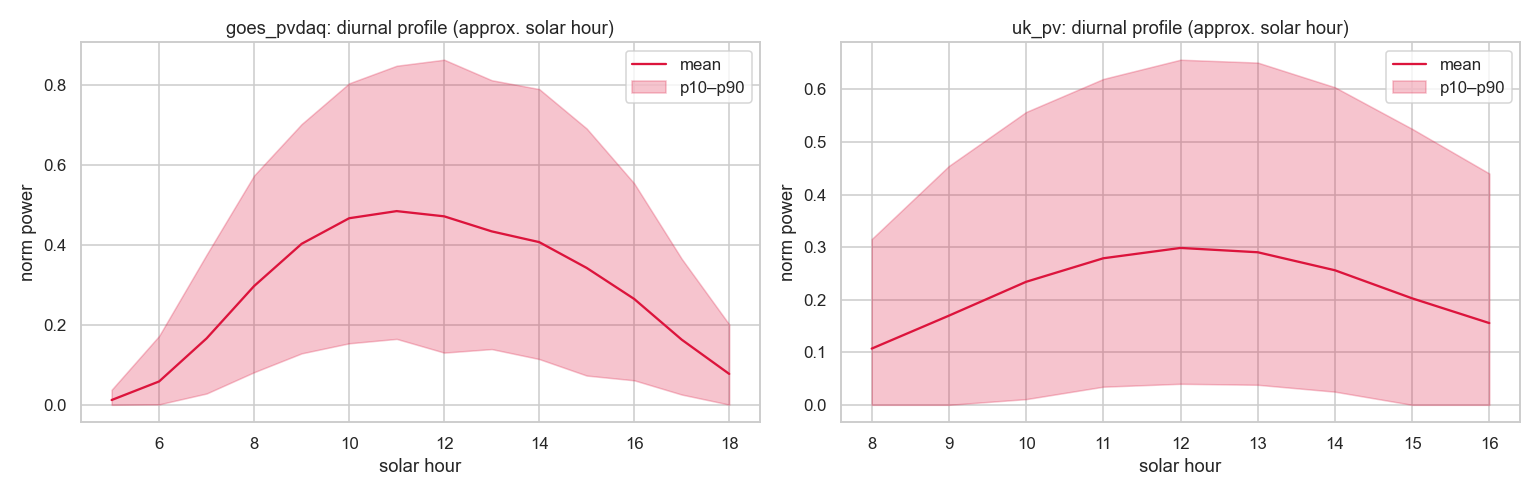
\includegraphics[width=\textwidth]{figures/diurnal_profile.png}
\caption{Mean capacity-normalised power against solar hour, with the 10th--90th percentile
band, for both tracks. The mean is a smooth deterministic arc --- which a clear-sky model
captures for free --- while the band is enormous: at solar noon the tenth percentile of
\texttt{uk\_pv} output is near zero and the ninetieth is above 0.65. Essentially all of the
forecasting difficulty lives in that band, not in the mean, which is precisely why smart
persistence rather than climatology is the reference the skill score is defined against.}
\label{fig:diurnal}
\end{figure}

\begin{figure}[h!]
\centering
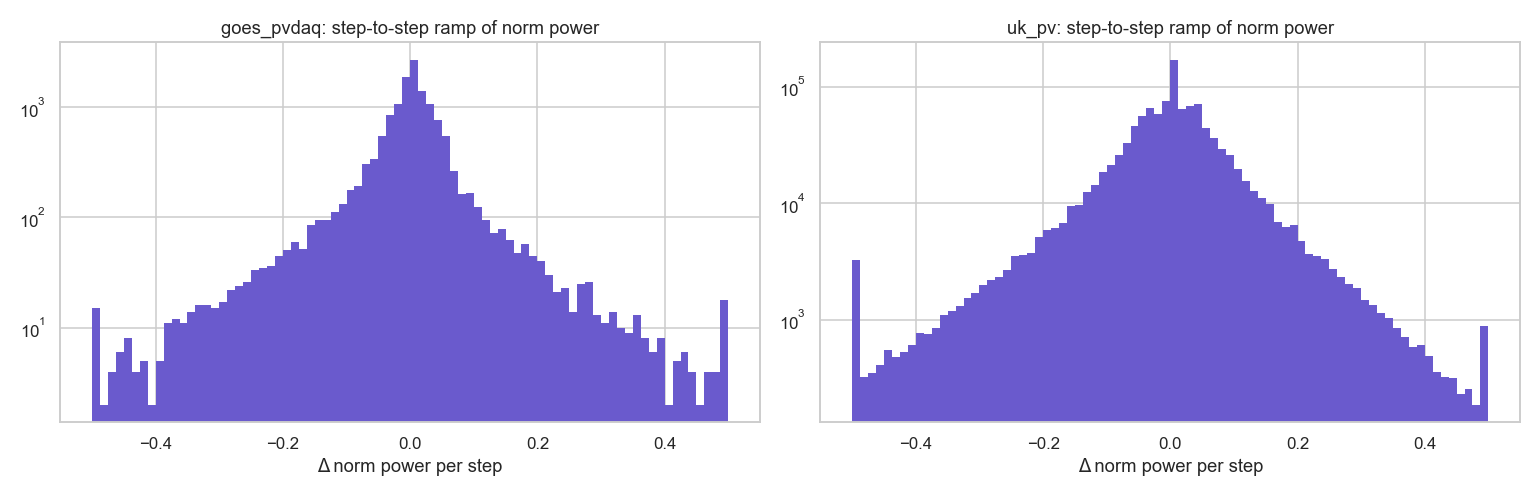
\includegraphics[width=\textwidth]{figures/ramp_rates.png}
\caption{Distribution of step-to-step changes in normalised power (logarithmic counts). The
distribution is sharply peaked at zero with heavy, near-exponential tails --- the signature
of a signal that is usually smooth and occasionally discontinuous. The ramp subset of
Section~\ref{sec:metrics} isolates the tails, which is where a visual modality is expected
to contribute and where persistence-like models fail.}
\label{fig:ramps}
\end{figure}

\begin{figure}[h!]
\centering
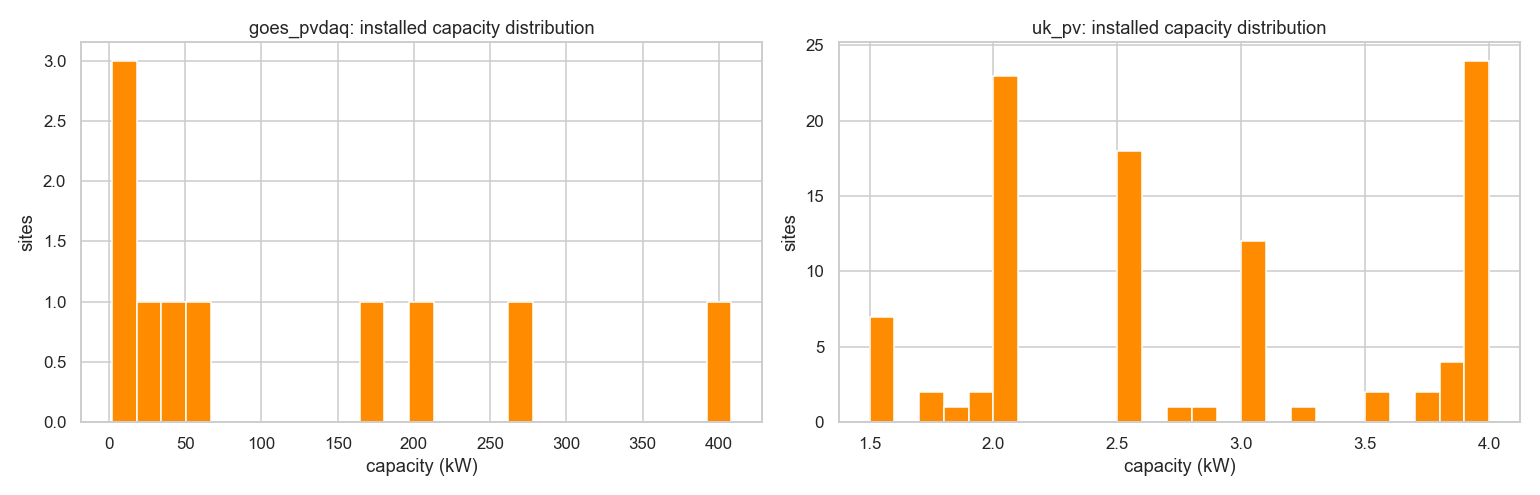
\includegraphics[width=\textwidth]{figures/capacity_distribution.png}
\caption{Installed capacity per site. \texttt{uk\_pv} is a narrow residential band clustered
at round values between 1.5 and 4.0\,kW; \texttt{goes\_pvdaq} spans more than two orders of
magnitude, from small residential systems to a 408\,kW array. Capacity normalisation is what
makes the two commensurable.}
\label{fig:capacity}
\end{figure}

\begin{figure}[h!]
\centering
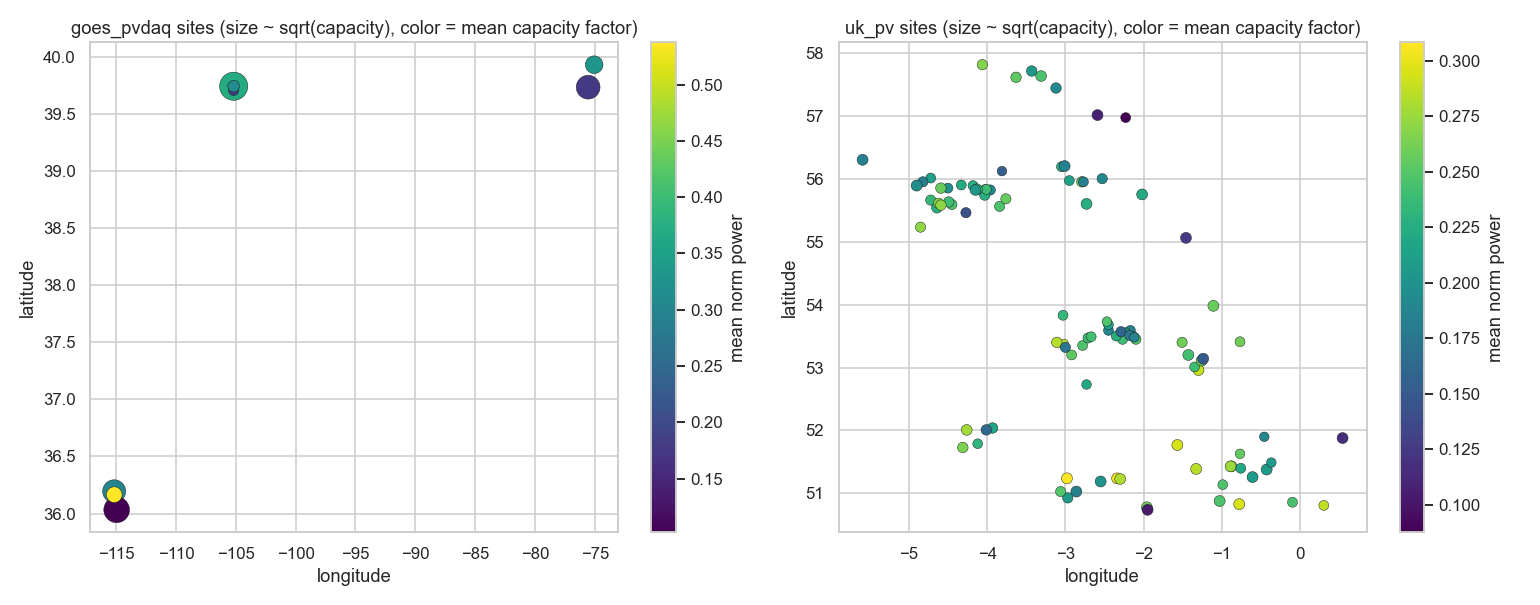
\includegraphics[width=\textwidth]{figures/site_map.png}
\caption{Site locations, sized by capacity and coloured by mean capacity factor. The
\texttt{uk\_pv} fleet is spatially dense: many sites are within tens of kilometres of each
other and therefore share a cloud field. This is the geometry behind the spatial-leakage
caveat of Section~\ref{sec:splits} --- a random plant split does not guarantee spatial
separation. Note also the systematic north--south gradient in capacity factor, a
generalisation axis a cross-plant model must absorb.}
\label{fig:sitemap}
\end{figure}

The two tracks differ in almost every respect that matters for generalisation, which is
what makes their combination valuable. \texttt{uk\_pv} is a dense fleet of 100 residential
rooftop systems between 1.5 and 4.0\,kW, confined to a small geographic envelope (latitude
50.7--57.8, longitude $-5.6$--$0.5$) and observed through a single-channel high-resolution
visible product. \texttt{goes\_pvdaq} spans capacities from 1.8 to 408\,kW --- residential
through utility scale --- across a continental spread of the United States (latitude
36.0--39.9, longitude $-115.2$--$-75.0$), observed in three-channel RGB at twice the
temporal cadence but over nine months rather than two years. A model that transfers between
them is transferring across sensor, scale, climate and cadence simultaneously.

\section{Exploratory analysis}
\label{sec:eda}

This section characterises the signal a forecaster has to model. It is not a formality: three
of the design decisions defended elsewhere in this thesis --- the choice of smart persistence
as the reference, the decision to keep a short visual window, and the expectation that vision
should matter in the ramp regime --- rest on properties visible here and nowhere else.

\subsection{The signal is a deterministic envelope plus a stochastic modulation}

Figure~\ref{fig:weektrace} makes the structure of the problem concrete over a single week.
Shortwave radiation (blue) traces smooth, nearly symmetric daily arcs whose amplitude varies
with season and synoptic conditions. Measured power (red) follows the same envelope but is
persistently rougher: on 05 and 07 January the power curve collapses to a fraction of what
the radiation curve implies; on 10 and 19 January the two agree closely; and on several days
the power series oscillates at high frequency within a single afternoon while the radiation
series --- which is hourly reanalysis interpolated to the power grid --- stays smooth.

That mismatch is the forecasting problem in one picture. The deterministic part of the signal
is nearly free: solar geometry gives it analytically. The residual is what the model must
predict, it lives at a temporal scale finer than the reanalysis resolves, and it is driven by
cloud structure that is not represented in any numerical channel at that resolution.

\begin{figure}[h!]
\centering
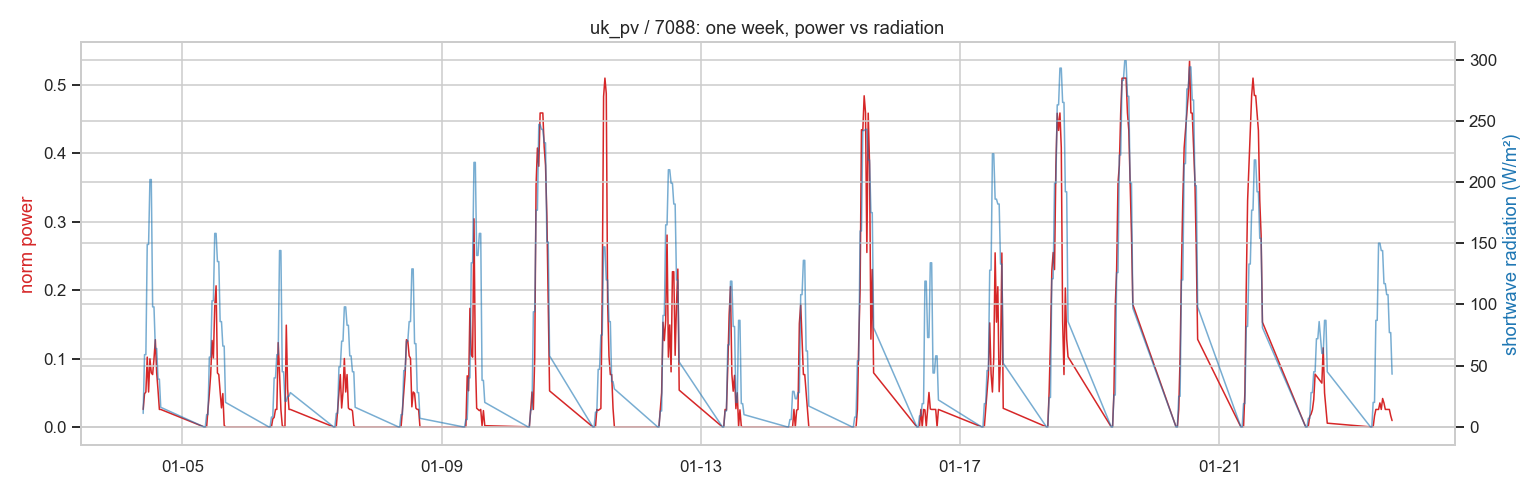
\includegraphics[width=\textwidth]{figures/week_uk_pv.png}
\caption{One week at a single \texttt{uk\_pv} site: normalised power (red, left axis) against
shortwave radiation (blue, right axis). The radiation channel is hourly reanalysis and is
consequently smooth; power varies at the native 30-minute cadence and frequently departs from
the envelope the radiation implies. The gap between the two curves is what a forecaster must
model, and it is finer-grained than the covariate track can express.}
\label{fig:weektrace}
\end{figure}

\subsection{The mean is trivial; the spread is the problem}

Figure~\ref{fig:diurnal} already showed that the conditional mean is a smooth arc with an
enormous percentile band around it. Figure~\ref{fig:monthhour} extends this to the seasonal
axis. For \texttt{uk\_pv} the mean normalised power is an almost perfectly separable function
of month and solar hour: a bright core around April to July at solar noon, decaying
symmetrically in both directions, with the winter months (November to January) contributing
almost nothing at any hour. The pattern is so regular that a lookup table indexed by month
and hour --- the hourly climatology baseline --- reaches a skill score of 0.234 without
observing the current day at all.

The consequence for evaluation is direct. A metric computed against a reference that does
\emph{not} know the diurnal and seasonal structure rewards a model mostly for rediscovering
astronomy. This is precisely why the skill score in Section~\ref{sec:metrics} is defined
against smart persistence, which is given the clear-sky curve, rather than against naive
persistence or against zero.

\begin{figure}[h!]
\centering
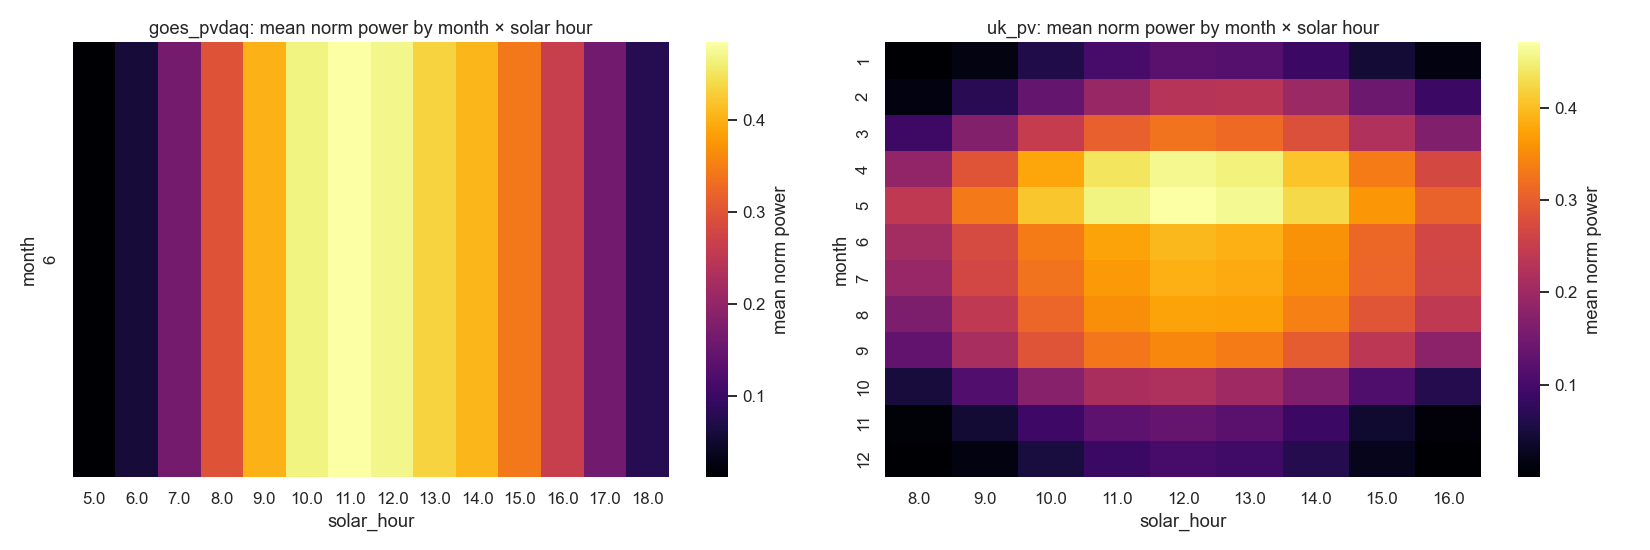
\includegraphics[width=\textwidth]{figures/month_hour_heatmap.png}
\caption{Mean normalised power by month and solar hour. The \texttt{uk\_pv} panel (right) is
close to separable in its two arguments --- a strong, entirely deterministic seasonal and
diurnal structure that any competent model captures and that therefore carries no
discriminative information between models. The \texttt{goes\_pvdaq} panel (left) covers a
single month and shows the diurnal axis only.}
\label{fig:monthhour}
\end{figure}

\subsection{Predictability decays within the forecast horizon}

Figure~\ref{fig:acf} plots the autocorrelation of normalised power against lag in hours. Two
readings matter. First, correlation falls below 0.5 within roughly three hours on
\texttt{uk\_pv} and within two on \texttt{goes\_pvdaq} --- comfortably inside the six-hour
horizon this thesis forecasts. The task is genuinely hard at the horizon chosen: half the
linear predictability is gone before the horizon is half over. Second, the two datasets
behave very differently at longer lags. \texttt{uk\_pv} autocorrelation flattens near 0.35
and then \emph{rises} again towards 0.45 around eight hours, the signature of the diurnal
cycle folding back; \texttt{goes\_pvdaq} plunges to $-0.75$ at six hours, which is what a
single-peaked daily arc produces when the lag reaches the half-period. The difference is a
cadence and latitude effect, and it is a concrete illustration of why metrics are never
pooled across the two tracks (Section~\ref{sec:windows}).

\begin{figure}[h!]
\centering
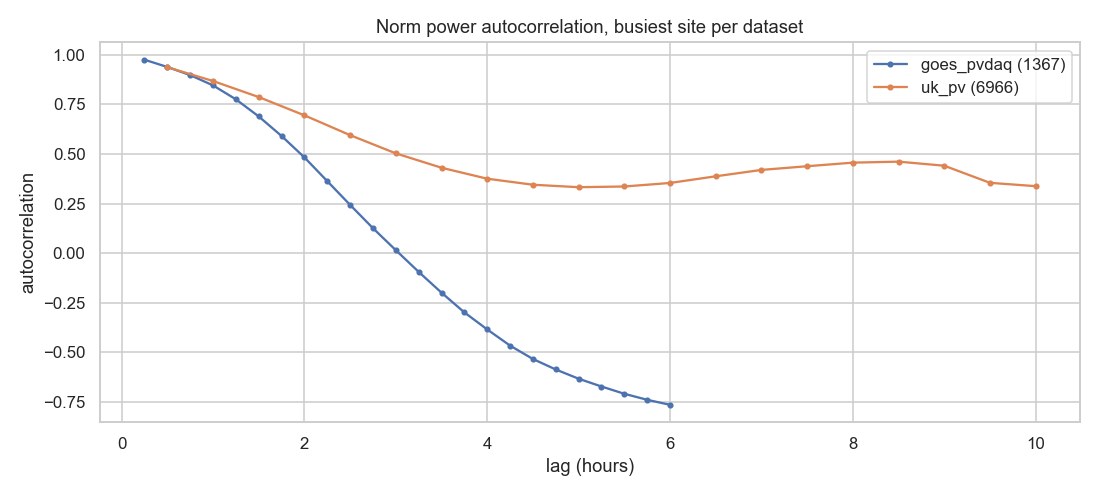
\includegraphics[width=0.85\textwidth]{figures/power_acf.png}
\caption{Autocorrelation of normalised power against lag in hours, busiest site per dataset.
Linear predictability halves within two to three hours --- well inside the six-hour forecast
horizon. The negative excursion on \texttt{goes\_pvdaq} is the half-period of the diurnal
arc, not a modelling artefact.}
\label{fig:acf}
\end{figure}

\subsection{Ramps are rare, large, and where the difficulty concentrates}

Figure~\ref{fig:ramps} showed the step-to-step change distribution: sharply peaked at zero
with heavy, near-exponential tails on a logarithmic count axis. Most steps are nearly
constant; a small minority move by a third of nameplate capacity in a single interval. A
model optimised for average error can ignore the tails almost entirely and still score well,
which is exactly why the ramp subset of Section~\ref{sec:metrics} exists as a separate
reporting column. The spikes at the extremes of both panels are the clipping bounds of the
histogram, not a physical accumulation.

\subsection{Covariate structure: strong, redundant, and incomplete}

Figure~\ref{fig:correlations} gives the Pearson and Spearman correlation structure over
daytime rows. Three observations shape the modelling.

The covariates are \emph{strong}: normalised power correlates at 0.74 with shortwave
radiation, 0.69 with direct radiation and 0.60 with direct normal irradiance. A model with
access to the covariate track starts from a substantial advantage over one restricted to the
power history --- which is visible in the leaderboard, where every covariate-consuming model
outranks DLinear.

The covariates are \emph{redundant}: shortwave and direct radiation correlate at 0.93 with
each other, and direct normal irradiance with cloud cover at $-0.70$. There are not eight
independent weather channels here; there are perhaps three degrees of freedom presented eight
ways. This is the structure that variate-attention architectures exploit and that
channel-independent ones cannot, and it is the most plausible explanation for the ordering
between iTransformer and PatchTST in Chapter~\ref{cha:benchmark}.

The covariates are \emph{incomplete}, which is the point that motivates the entire visual
branch of this thesis. Figure~\ref{fig:hexbin} shows the joint density of power against each
driver. The relationship with shortwave radiation is broad rather than tight: at
400\,W/m$^2$ observed power ranges over most of the unit interval. Cloud cover, remarkably,
shows almost no marginal relationship at all --- the density is nearly uniform in the
horizontal direction --- because cloud cover as an hourly areal fraction says little about
whether the sun is occluded at a specific site at a specific minute.

\begin{figure}[h!]
\centering
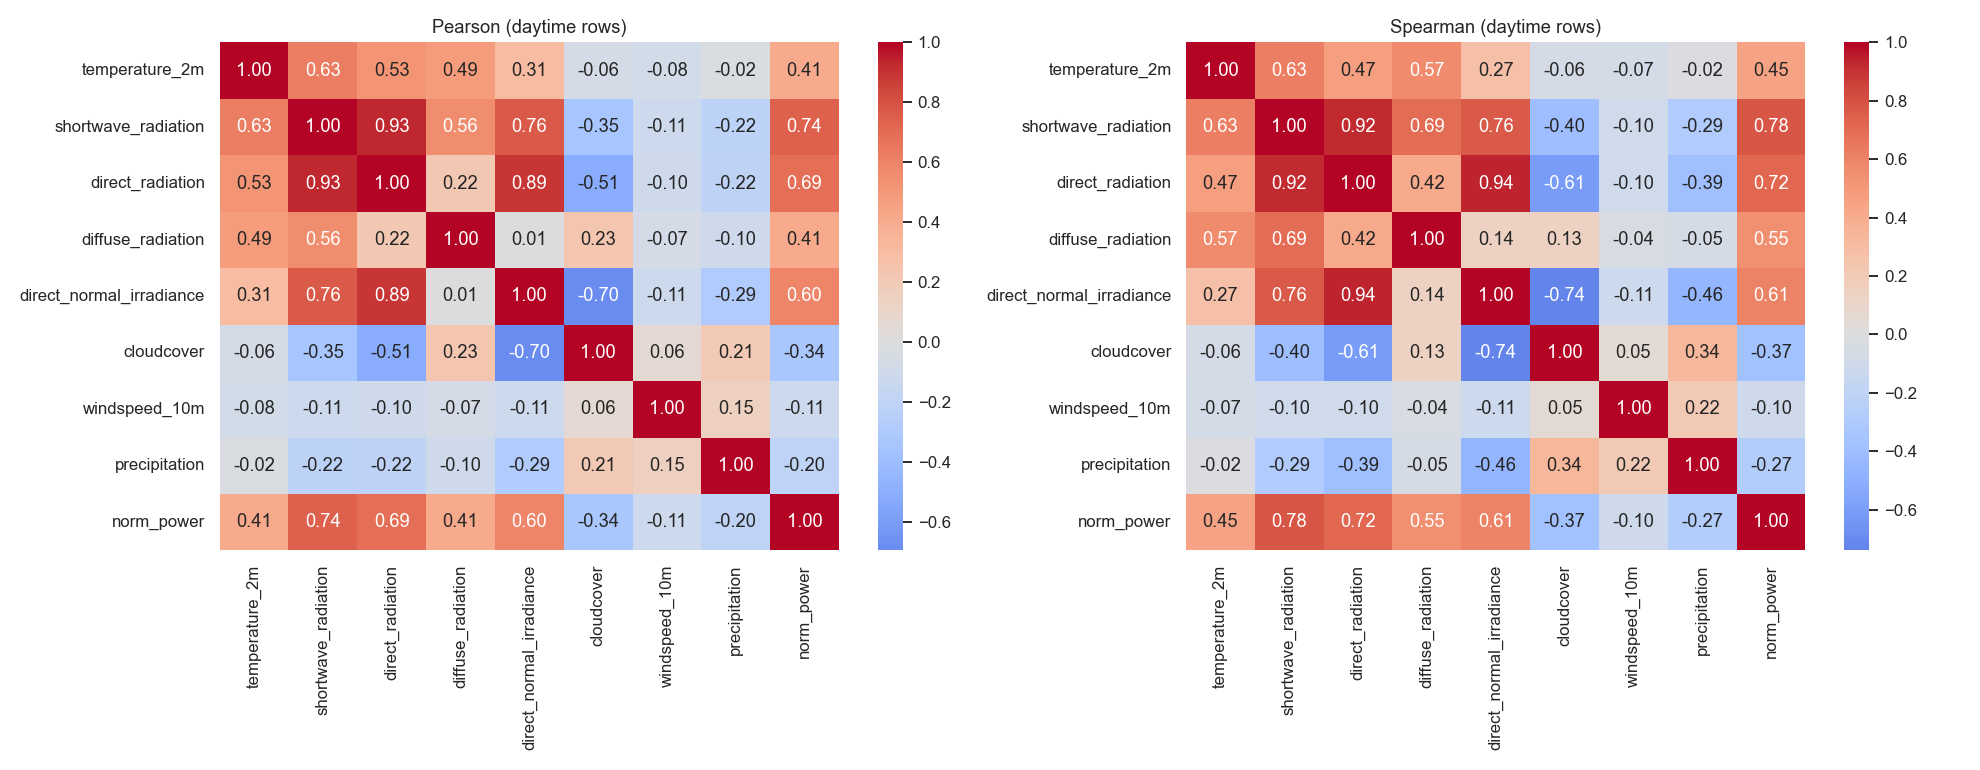
\includegraphics[width=\textwidth]{figures/correlation_matrices.png}
\caption{Pearson (left) and Spearman (right) correlation over daytime rows. The covariate
block is strongly inter-correlated --- 0.93 between shortwave and direct radiation --- so the
effective dimensionality of the weather track is far below its eight channels.}
\label{fig:correlations}
\end{figure}

\begin{figure}[h!]
\centering
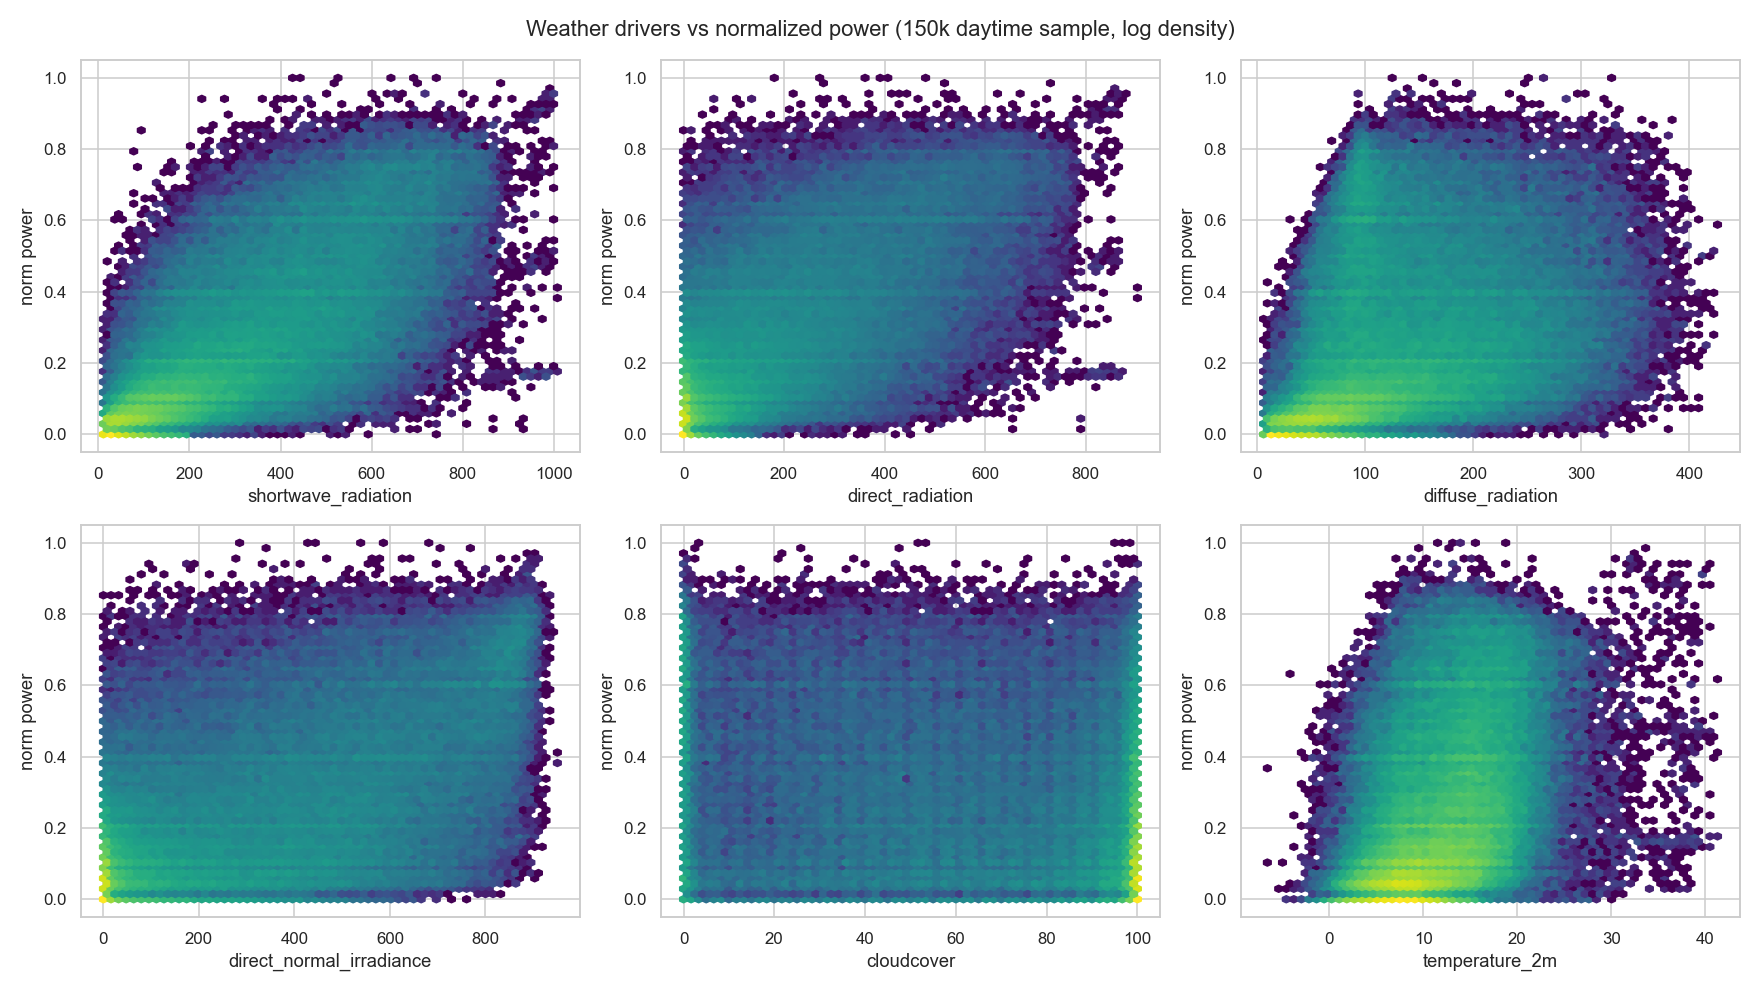
\includegraphics[width=\textwidth]{figures/feature_vs_power_hexbin.png}
\caption{Joint density of normalised power against each weather driver (logarithmic density,
150k daytime sample). The irradiance panels show broad, cone-shaped relationships rather than
tight ones; the cloud-cover panel is nearly uninformative marginally, because an hourly areal
cloud fraction does not determine occlusion at a point.}
\label{fig:hexbin}
\end{figure}

\subsection{There is residual cloud information beyond irradiance}

Figure~\ref{fig:cloud-residual} isolates the effect that motivates a visual modality. Daytime
observations are binned by shortwave radiation, and within each bin further split by cloud
cover. If the reanalysis irradiance already captured the cloud state, the three boxes within
a bin would coincide. They do not. In the 250--450\,W/m$^2$ bin the median falls from 0.33
under clear skies to 0.27 under mixed conditions to 0.24 under overcast, and the same
monotone ordering holds in every bin. Conditioning on cloud state adds information
\emph{after} conditioning on irradiance.

This is the empirical case for the thesis. There exists cloud-state information not carried
by the numerical channels, it is exactly the kind of information a satellite crop observes
directly, and the size of the effect --- roughly 0.09 in normalised power at fixed irradiance
--- is of the same order as the differences separating models in the leaderboard.
Chapter~\ref{cha:benchmark} reports that no model consuming real frames converts this into
skill, which makes the figure the sharpest statement of the gap between what is available and
what is exploited.

\begin{figure}[h!]
\centering
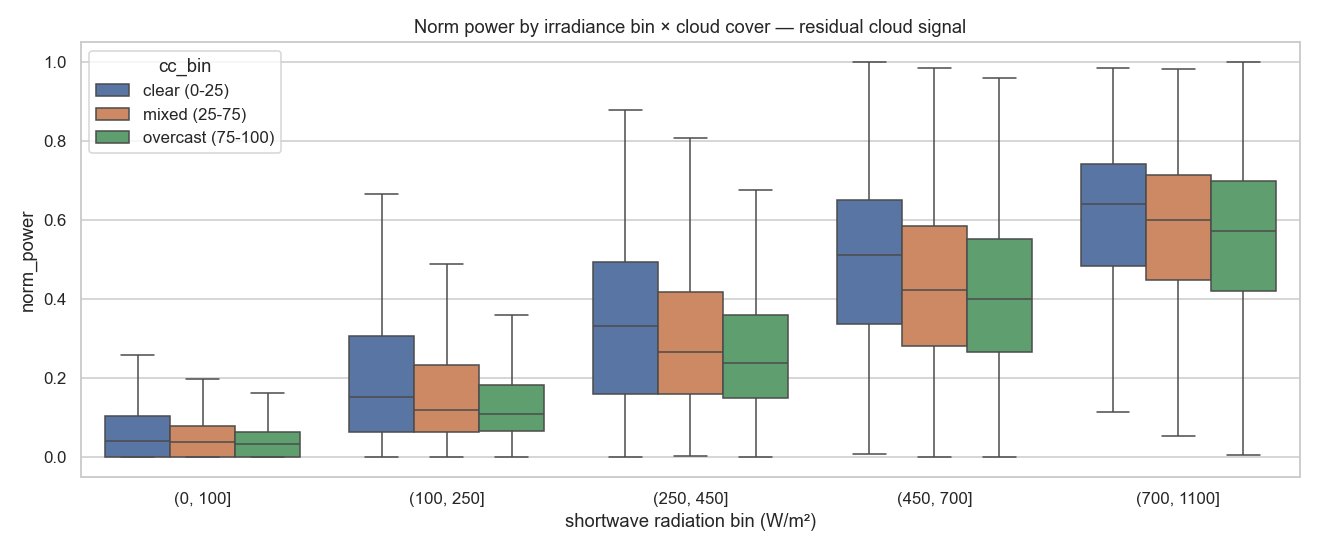
\includegraphics[width=\textwidth]{figures/cloudcover_residual_effect.png}
\caption{Normalised power by irradiance bin, split by cloud cover within each bin. The
monotone separation of the three boxes at fixed irradiance is residual cloud-state
information that the numerical covariate track does not carry --- and that a satellite frame
observes directly.}
\label{fig:cloud-residual}
\end{figure}

\subsection{The second track behaves differently}

Figure~\ref{fig:weekgoes} shows the same week-long view for a \texttt{goes\_pvdaq} site. The
contrast with Figure~\ref{fig:weektrace} is the reason the two tracks are kept separate in
every table. The cadence is twice as fast, the capacity factor is markedly higher, the daily
arcs are broader --- a lower-latitude summer --- and the power curve tracks the radiation
envelope more closely, with fewer of the deep intra-day collapses that characterise the UK
fleet.

A model that transfers between these tracks is transferring across sensor (greyscale
high-resolution visible against three-channel GOES), spatial scale (a 128\,km crop at 1\,km
resolution against a 256-pixel RGB frame), capacity class (kilowatts against hundreds of
kilowatts), climate, latitude and sampling cadence simultaneously. That is a genuine
distribution shift and the reason scenario S3 is the strongest available test of
generalisation --- and the reason its absence from the executed scenarios is the principal
limitation of this work.

\begin{figure}[h!]
\centering
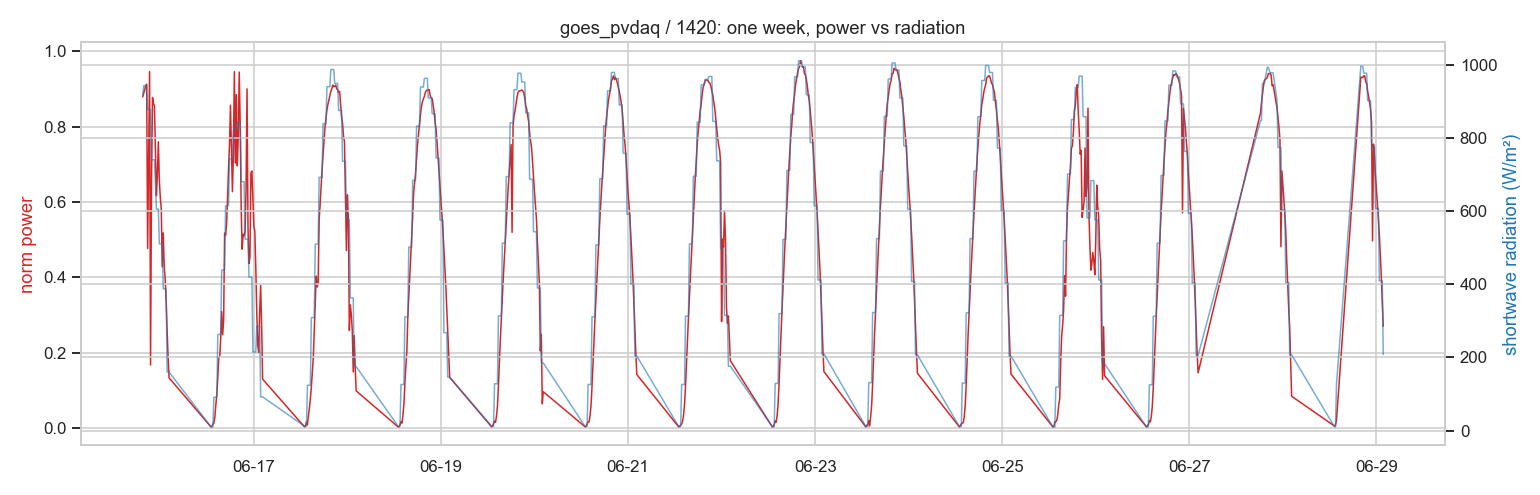
\includegraphics[width=\textwidth]{figures/week_goes_pvdaq.png}
\caption{One week at a \texttt{goes\_pvdaq} site, at 15-minute cadence. Compare
Figure~\ref{fig:weektrace}: higher capacity factor, broader arcs, closer tracking of the
radiation envelope. The two tracks are different forecasting problems sharing a schema.}
\label{fig:weekgoes}
\end{figure}

\subsection{Between-plant heterogeneity}

Figure~\ref{fig:siteboxplot} shows the distribution of daytime normalised power per site.
Even after capacity normalisation, medians range from below 0.10 to above 0.55, and the
inter-quartile ranges differ by a factor of three. Part of this is geography --- the
north--south gradient visible in Figure~\ref{fig:sitemap} --- and part is per-installation
factors that the dataset does not record: tilt, azimuth, shading, module technology,
inverter clipping behaviour.

This heterogeneity is what makes cross-plant transfer non-trivial and what a temporal split
would hide entirely. A model fitted on one plant and tested on the same plant absorbs its
orientation and shading into its parameters; a model that must generalise across plants
cannot, and has to recover whatever is recoverable from a two-week history at inference
time. The \texttt{goes\_pvdaq} sites (orange) sit systematically higher, reflecting both
lower latitude and a different mix of installation types --- which is why cross-dataset
transfer is a genuine distribution shift and not a formality.

\begin{figure}[h!]
\centering
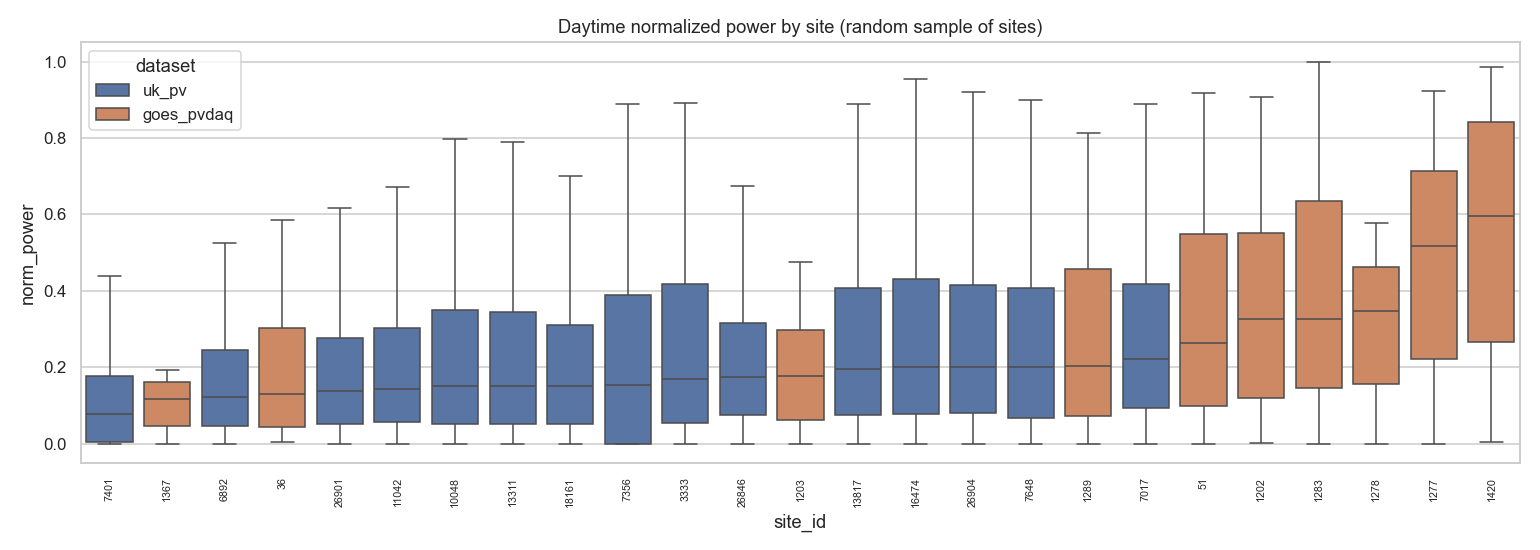
\includegraphics[width=\textwidth]{figures/site_norm_power_boxplot.png}
\caption{Daytime normalised power by site, random sample of sites from both tracks. Capacity
normalisation removes the scale difference but not the difference in \emph{capacity factor};
the residual spread is the between-plant variation a cross-plant model must absorb.}
\label{fig:siteboxplot}
\end{figure}

\subsection{The target distribution is zero-inflated and right-skewed}

Figure~\ref{fig:powerdist} shows why the target is awkward for a general-purpose sequence
model. Over all rows the distribution has a dominant spike at zero --- night, outage and
deep-overcast steps --- and a long right tail that never approaches the theoretical maximum
of one. Restricting to production steps removes the spike but leaves a strongly right-skewed
distribution with most mass below 0.3. In absolute units the picture is different again:
log-power is roughly bimodal, reflecting the two capacity populations of the two tracks.

Three modelling consequences follow. A model whose output head assumes an unbounded,
approximately symmetric predictive distribution --- as most general-purpose foundation model
heads do --- is mismatched at both ends: it can predict negative power, and it wastes
probability mass above the observed ceiling. The zero spike means that a large fraction of
the loss is contributed by observations that are trivially predictable given solar geometry,
which inflates apparent accuracy unless evaluation is restricted to daylight steps --- as it
is here. And the right skew means mean-squared objectives are dominated by a minority of
high-output steps, which is one reason NMAE and NRMSE order models differently in
Chapter~\ref{cha:benchmark}.

\begin{figure}[h!]
\centering
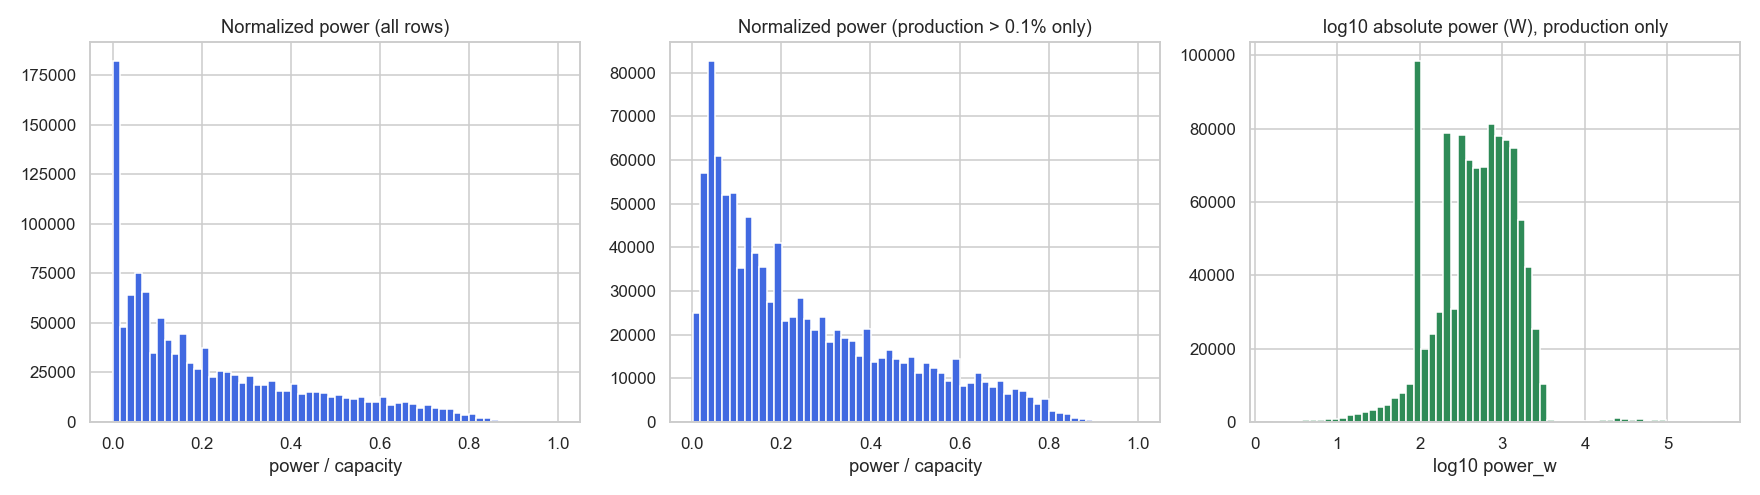
\includegraphics[width=\textwidth]{figures/power_distributions.png}
\caption{Target distribution. Left: all rows, showing the dominant zero spike. Centre:
production steps only, right-skewed with most mass below 0.3 and an effective ceiling near
0.85 rather than 1.0. Right: $\log_{10}$ absolute power, whose bimodality reflects the two
capacity populations.}
\label{fig:powerdist}
\end{figure}

\subsection{Per-plant driver relationships are stable}

Figure~\ref{fig:capfactor} decomposes the between-plant variation of
Figure~\ref{fig:siteboxplot} into two histograms. Daytime mean capacity factor is tightly
concentrated for \texttt{uk\_pv} --- most sites between 0.20 and 0.32 --- with the
\texttt{goes\_pvdaq} sites spread much wider and reaching 0.54. But the per-site correlation
between normalised power and shortwave radiation is remarkably consistent: nearly every
\texttt{uk\_pv} site falls between 0.70 and 0.87, and the \texttt{goes\_pvdaq} sites reach
0.94.

This is the empirical basis for believing cross-plant transfer is possible at all. Plants
differ substantially in their \emph{level} --- how much they produce --- but very little in
the \emph{structure} of their response to the dominant driver. A model that learns the
irradiance-to-power relationship on one fleet has learned something that holds on another;
what it cannot carry over is the plant-specific scaling, which is exactly what the short
inference history is there to supply.

\begin{figure}[h!]
\centering
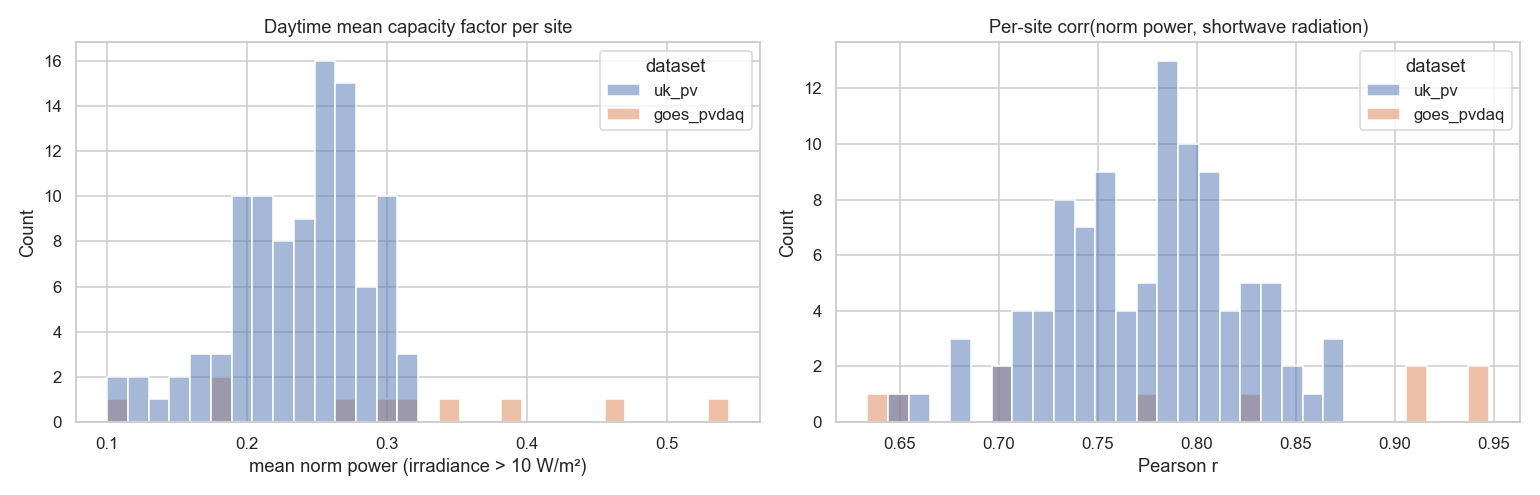
\includegraphics[width=\textwidth]{figures/site_capacity_factor_and_corr.png}
\caption{Left: daytime mean capacity factor per site. Right: per-site Pearson correlation
between normalised power and shortwave radiation. Levels differ substantially across plants;
the structure of the driver relationship barely does. Cross-plant transfer is a problem of
recovering level, not of relearning structure.}
\label{fig:capfactor}
\end{figure}

\subsection{Coverage and missingness}

Figure~\ref{fig:availability} shows per-site data availability by month. Coverage is dense
but not complete: a minority of sites begin reporting only in mid-2019, and a few have
interior gaps. Nothing is imputed across these gaps --- windows that would span one are
simply not generated --- which keeps the evaluation honest at the cost of a slightly uneven
sampling of forecast origins across sites.

The structural missingness matters more than the incidental kind. Night steps have no
frames at all, and outage and stuck-sensor rows are masked out of the target. The visual
mask is therefore correlated with time of day by construction, and any model consuming the
visual stream must handle a systematically absent modality rather than a randomly absent
one. This is the reason modality dropout is part of the tensor contract of
Section~\ref{sec:contract} rather than a training-time detail.

\begin{figure}[h!]
\centering
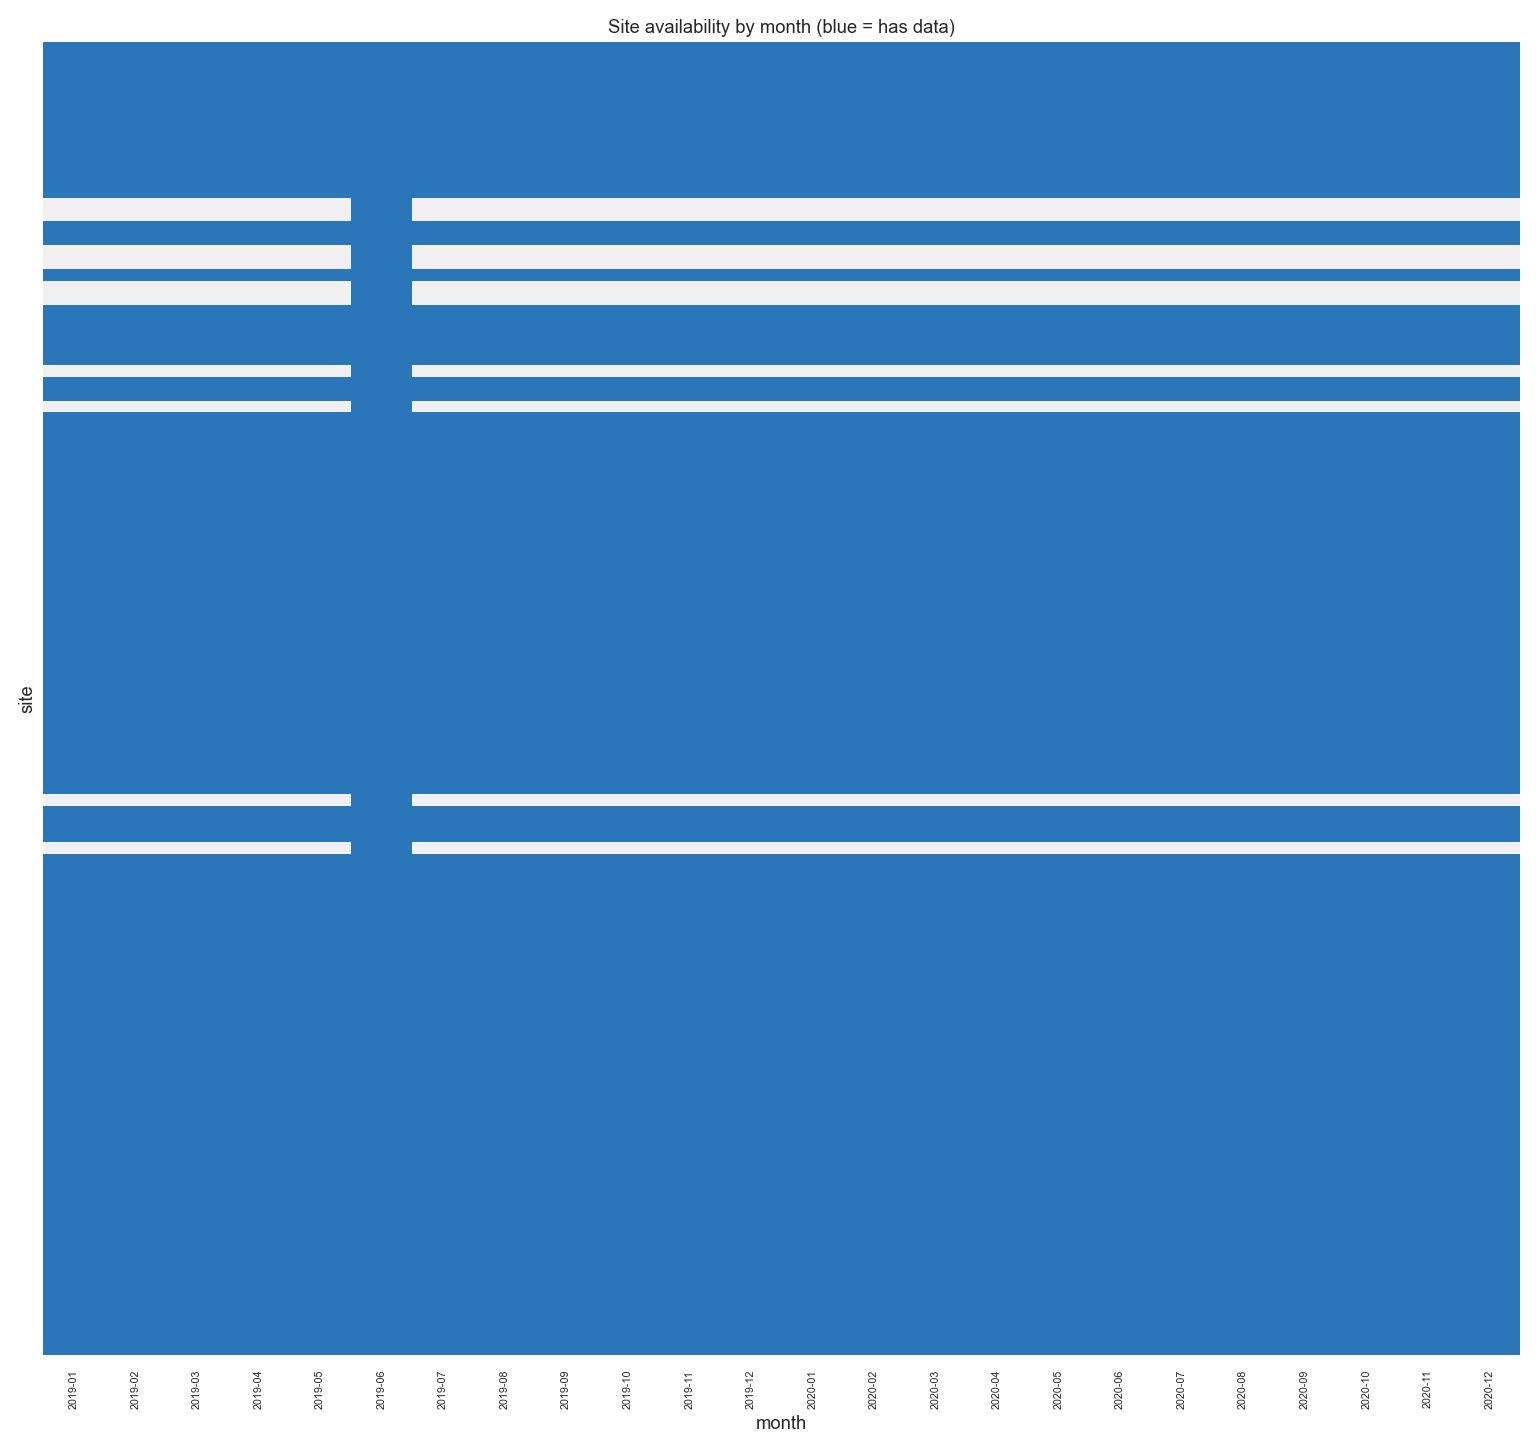
\includegraphics[width=0.78\textwidth]{figures/site_availability_timeline.png}
\caption{Per-site availability by month (blue indicates data present). Coverage is broadly
dense; a minority of sites start mid-2019 or carry interior gaps. No values are imputed
across gaps --- affected windows are not generated.}
\label{fig:availability}
\end{figure}

Quantitatively, coverage is better than the timeline suggests. Figure~\ref{fig:coverage}
shows the fraction of days within each site's span that carry data: every \texttt{uk\_pv} site
exceeds 99.3 percent, and forty-four of them are complete. The gaps visible in
Figure~\ref{fig:availability} are therefore late \emph{starts} rather than interruptions ---
a set of sites that joined the fleet mid-2019 --- which affects how many windows a site
contributes but not the continuity of the windows it does contribute.

\begin{figure}[h!]
\centering
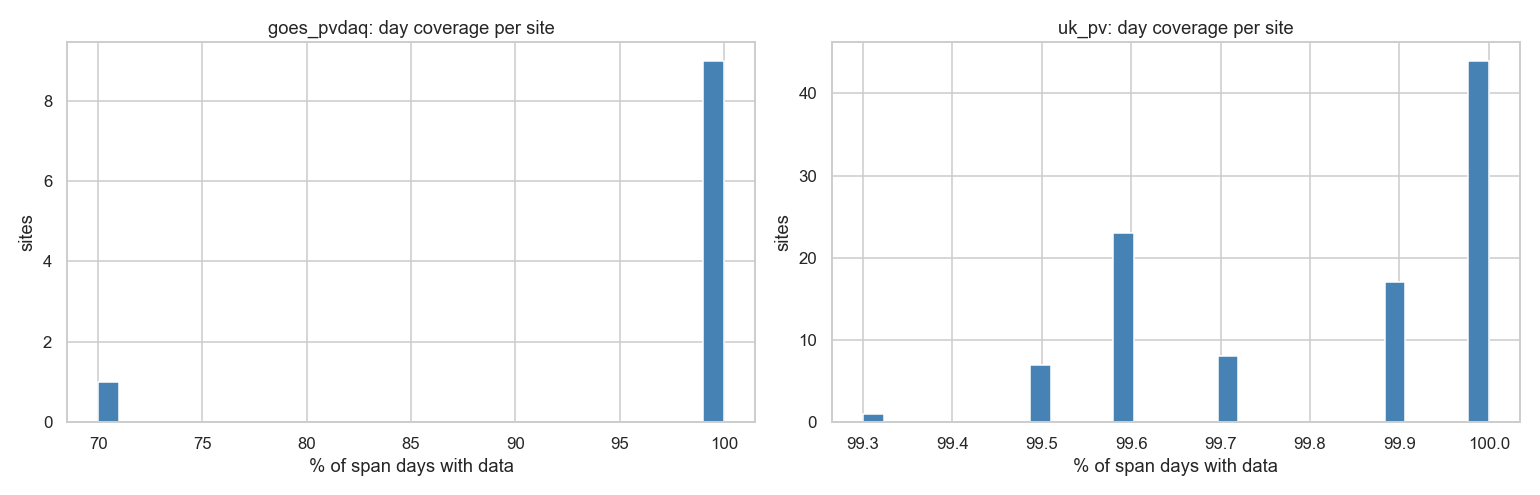
\includegraphics[width=\textwidth]{figures/coverage_per_site.png}
\caption{Percentage of days within each site's span that carry data. Coverage exceeds 99.3
percent for every \texttt{uk\_pv} site. The apparent gaps in Figure~\ref{fig:availability} are
late starts, not interruptions.}
\label{fig:coverage}
\end{figure}

\subsection{Seasonality and the two-year span}

Figure~\ref{fig:monthly} shows mean normalised power by calendar month across the full
\texttt{uk\_pv} span. The seasonal cycle is large --- a factor of eight between December
(0.05) and May (0.42) --- and it repeats closely across the two years, with 2020 running
slightly higher in spring than 2019.

Two consequences for evaluation follow. Because the split is by plant rather than by time,
every plant contributes windows from every season, so no model is advantaged by a favourable
temporal slice; the seasonal cycle is common-mode across train, validation and test. And
because the span covers two full years, the seasonal cycle is observed twice, which is the
minimum required for a fourteen-day context window to be interpretable: with a single year, a
model could not distinguish a seasonal trend from a secular one. The single-month
\texttt{goes\_pvdaq} overlap point is a reminder that the second track covers only nine
months and cannot support the same seasonal analysis.

\begin{figure}[h!]
\centering
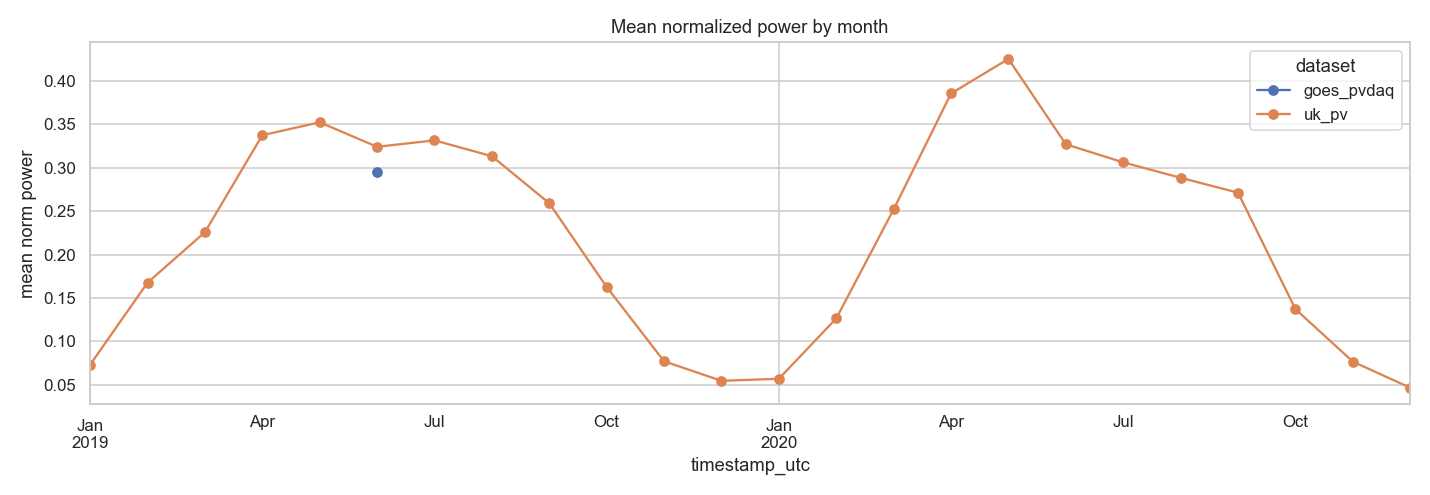
\includegraphics[width=\textwidth]{figures/monthly_production.png}
\caption{Mean normalised power by month over the full span. The seasonal cycle spans a factor
of eight and repeats closely across the two years. Plant-based splitting makes this cycle
common-mode across train, validation and test.}
\label{fig:monthly}
\end{figure}

\section{Splits}
\label{sec:splits}

Splits partition \emph{plants}, are generated once with seed 42 at a per-dataset
70/15/15 ratio, exclude sites carrying \texttt{bad\_site\_flag}, and are committed to a
version-controlled file. Disjointness is asserted programmatically at every data load
rather than trusted; a leak would raise rather than silently improve a score.

\begin{table}[h!]
\centering
\small
\begin{tabular}{l c c c p{5.2cm}}
\hline
\textbf{Role} & \textbf{Plants} & \textbf{Rows} & \textbf{Valid steps} & \textbf{Purpose} \\
\hline
Train & 69 & 850{,}654 & 846{,}633 & Fit parameters, fine-tune backbones \\
Validation & 15 & 184{,}899 & 182{,}809 & Early stopping, hyperparameter and mixing-weight
tuning \\
Test & 14 & 172{,}656 & 171{,}543 & Final reporting only \\
Excluded & 2 & --- & --- & \texttt{bad\_site\_flag}: sites 7239, 8587 \\
\hline
\end{tabular}
\caption{The \texttt{uk\_pv} plant partition. Exact site membership is listed in
Appendix~\ref{app:splits}.}
\label{tab:splits}
\end{table}

The companion \texttt{goes\_pvdaq} split is 7 train / 2 validation / 1 test. With ten
plants, a fixed 15\% test share is one or two plants, and per-plant variance would dominate
any comparison; that track is therefore additionally evaluated \emph{leave-one-plant-out},
reporting mean and standard deviation over folds.

\paragraph{A limitation of random plant assignment.} Assigning plants to splits at random
does not guarantee \emph{spatial} disjointness. Two \texttt{uk\_pv} rooftops a few
kilometres apart experience nearly the same cloud field, so a random split can place a test
plant's near-twin in the training set and leak spatial information that a
distance-based or region-based split would withhold. The split used here is random because
it is the convention the baseline literature follows and because changing it mid-study
would invalidate cross-comparison; a region-based variant is identified as future work in
Section~\ref{sec:future}. The effect is expected to inflate all models equally rather than
to favour any particular one, but it inflates the absolute numbers.

\section{The tensor contract}
\label{sec:contract}

Every model in this thesis --- baselines and proposed architecture alike --- consumes the
same dictionary emitted by the dataset adapter. Fixing this contract is what makes the
comparison of Chapter~\ref{cha:baselines} a comparison of \emph{models} rather than of data
pipelines. With $N$ entities, history $T$, horizon $H$ and $T_v$ frames:

\begin{table}[h!]
\centering
\small
\begin{tabular}{l l l}
\hline
\textbf{Key} & \textbf{Shape} & \textbf{Content} \\
\hline
\texttt{Y} & $(N, T, C_{\text{tgt}})$ & Normalised historical target \\
\texttt{Y\_future} & $(N, H, C_{\text{tgt}})$ & Ground-truth horizon \\
\texttt{X\_cov} & $(N, T+H, C_{\text{cov}})$ & Historical and future covariates \\
\texttt{V} & $(N, T_v, C_{\text{img}}, H_{\text{img}}, W_{\text{img}})$ & Frames normalised
to $[0,1]$ \\
\texttt{timestamps} & $(T+H,)$ & Unix epoch over the full window \\
\texttt{timestamps\_v} & $(T_v,)$ & Unix epoch of the frames \\
\texttt{entity\_ids} & $(N,)$ & Plant identifiers \\
\texttt{mask\_target} & $(N, T, C_{\text{tgt}})$ & Validity of historical targets \\
\texttt{mask\_future} & $(N, H, C_{\text{tgt}})$ & Evaluation mask \\
\texttt{mask\_visual} & $(N, T_v)$ & Validity of each frame \\
\texttt{mask\_modality\_dropout} & $(N, 2)$ & Numeric / visual dropout \\
\texttt{adj\_matrix} & $(N, N)$ & Precomputed spatial adjacency \\
\hline
\end{tabular}
\caption{The canonical batch dictionary. All models read this and nothing else.}
\label{tab:contract}
\end{table}

\subsection{Notes for re-use}

Six points would save a future user of this dataset a considerable amount of time, and they
are collected here rather than scattered through the chapter.

\begin{enumerate}
  \item \textbf{Read frames only through \texttt{image\_h5\_index}}, and remember it is
    group-local. \texttt{image\_uk128\_index} is dead; \texttt{image\_index} is an
    approximation retained for compatibility.
  \item \textbf{Respect \texttt{bad\_site\_flag}} before generating splits. The committed
    \texttt{goes\_pvdaq} partition predates the flags and must be regenerated.
  \item \textbf{Do not standardise per series.} Use capacity normalisation; anything
    estimated from the series leaks under a cross-plant protocol.
  \item \textbf{Distinguish zero from missing.} Night power is genuinely zero; outage power is
    absent. The masks carry the distinction and the target column does not.
  \item \textbf{Do not resample across tracks.} The two cadences are native and physical-time
    windows resolve to different step counts; pooling raw step-horizon metrics across them is
    a category error.
  \item \textbf{Expect a structurally missing visual stream.} There are no night frames, so
    visual availability is correlated with time of day by construction.
\end{enumerate}

Two design decisions in this contract are worth stating explicitly. Masks are carried
alongside the data rather than encoded as sentinel values, so that a model can distinguish
``zero power'' from ``no measurement'' --- a distinction that matters enormously at dawn and
dusk. And \texttt{mask\_modality\_dropout} is part of the contract rather than a training
detail, so that robustness to missing frames can be evaluated under exactly the mechanism
used during training.

\par

